%
%	Theorieteil
%

\pagebreak
\section{Management of Container Platforms in the Enterprise}

\onehalfspacing

\subsection{Key requirements for Kubernetes cluster in Enterprise IT}

Once you start the transition to cloud-native application development and introduce containers to your IT production, Day Two operations and security becomes the main concern.

One of the crucial components of security when running containers in production, according to NIST, is separation\footnote{Vgl. \textit{Souppaya, M. (2017)}: Application Container Security Guide \cite{sp800-190}}.

Segmentation of applications could be along the line of function (Production, Development/Test), or application, or both. Separation could be achieved in single cluster environments through networking or the introduction of multiple clusters. 

\begin{figure}[h]
\centering
\caption {Cluster Separation}
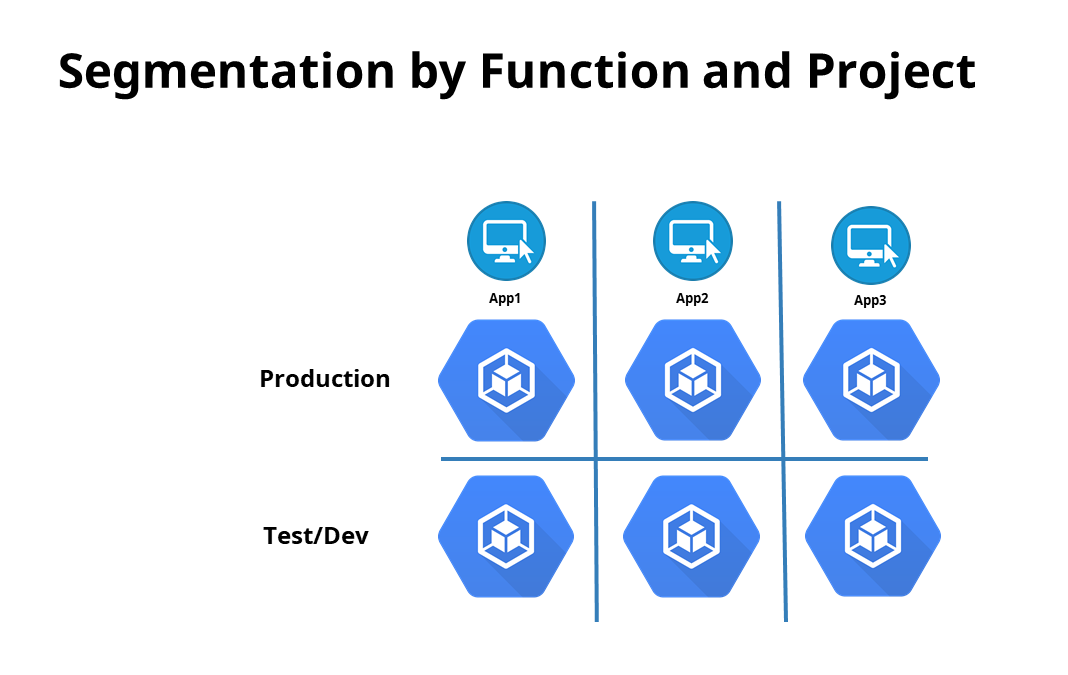
\includegraphics[width=\linewidth]{images/separation}
\label{fig:clusterSeparation}
\end{figure}

A key consideration when implementing separation is the so-called "Blast Radius", a term borrowed from the military, depicting the amount of damage an explosive would cause. In IT, it is used to assess the damage a breach, data loss, or failure of a certain IT system would cause to the whole operation, in technical and financial terms.

Defining application and data security classes is part of the preparation process when introducing containers to production, and would exceed the scope of this paper.

Kubernetes itself, at the time of writing, does not provide for hard tenancy. To fully separate applications on all layers (compute, network, and storage), the use of multiple clusters is a good option. Many enterprises might thus end up with more than one Kubernetes cluster, sometimes with many more, which will, in turn, have a great effect on operations.

\subsection{The principle of least privilege}

The second crucial component of security is user authentication and authorization.

Most Enterprise IT already have some form of central user authentication, through Microsoft Active Directory of other Single-Sign-On providers. Kubernetes has Role-Based Access Control and can restrict access to its resources based on the roles bound to a specific user or object.

Defining Roles and Responsibilities is part of the Role Engineering process during the introduction of containers, and would exceed the scope of this paper.

It is, however, important in RBAC to fully embrace the principle of least privilege - only ever grant the minimum access rights required to fulfill the job, without jeopardizing efficiency though.

\subsection{Other considerations}

The third crucial component of security is departmental organization - NIST recommends that an organization changes its operational culture and technical processes to fully embrace and support agile application development.

Without such changes, from experience, the likelihood of failing the transformation to container-based, cloud-native application development is quite high.

In Germany, BSI has published in 2018 a community draft of security guidelines for container run-time environments\footnote{Vgl. \textit{BSI (2018)}: SYS.1.6 Container \cite{sys16Container}}, which unfortunately focuses more on the theoretical and procedural application of security and includes very little actionable information.

\subsection{Day Two operations with multiple Kubernetai}

Once all preparations have been completed and multiple clusters are installed, there are a lot of configuration items and actions that need to be synchronized across all these clusters:

\begin{itemize}
\item User Authentication
\item Roles and Responsibilities
\item Security Policies
    \begin{itemize}
    \item Pod Security Policies
    \item Network Security Policies
    \end{itemize}
\item Version control and upgrades
    \begin{itemize}
    \item Kubernetes
    \item Applications
    \end{itemize}
\item Logging and Monitoring
\item Backup and Restore
\item Persistent volumes and storage classes
\end{itemize}

For software development and automatic deployment, it makes sense to connect your pipeline(s) to the respective clusters and establish central governance for the deployment workflows.

For micro-service observability, distributed tracing and network control, you would typically install a service mesh - one choice could be Istio\footnote{Vgl. \textit{Istio Authors (2019)}: Istio - Connect, secure, control, and observe services \cite{istio}}.

All of these tasks can be performed against individual clusters with native Kubernetes tools, but once you have a couple of them to manage, it will get tedious and quite difficult to synchronize.

It will even get more difficult, once you embrace IaC and try to treat your Kubernetes clusters as ephemeral, recreating the platform fresh with each new application deployment and relying on your automation to implement governance and policies.

\subsection{Possible solutions}

To address all these issues, CNCF is working on a multi-cluster controller, but it's still in its infancy and not production ready yet,

The three big cloud providers also provide solutions to manage multiple clusters: Google Cloud has Anthos\footnote{Vgl. \textit{Google (2019)}: Anthos - Bringing the cloud to you \cite{googleAnthos}}, Microsoft Azure has Azure Arc\footnote{Vgl. \textit{Microsoft (2019)}: Bring Azure services and management to any infrastructure \cite{azureArc}} in Preview, and AWS is working on AWS Outposts\footnote{Vgl. \textit{AWS (2019)}: AWS Outposts \cite{awsOutposts}}.

A popular open-source solution for this problem is Rancher\footnote{Vgl. \textit{Rancher Labs (2019)}: Run Kubernetes Everywhere \cite{rancher}}, by Rancher Labs. In the next chapter, we'll look at whether Rancher could provide a solution to multi-cluster management and become the tool of choice in Enterprise IT.
